% Chapter submission guide:
% https://docs.google.com/document/d/1Yui8fuxUEiMsIX2G-oKfUs3vObPXb2VzKi2CKvzAg3o/edit?tab=t.0

% Suggested length: 2-10 pages (500 words per page)
% = 1000 - 5000 words

% Chapter 1 example in PP book (Charlotte et al): 
% https://pairprogramming.ed.ac.uk/chapter-students-about-pair-programming/

\section{Introduction}
% What is this chapter? (very brief)

This chapter is designed to serve as a brief tour of connections between music and programming. In particular, it is aimed at educators who want to explore music in their pedagogy. The \href{}{accompanying resources} present a range of possible projects that can be adapted for classroom use or self-learning. 

Making code that makes sound and music can be fun, even with only a very basic understanding of programming concepts. It can motivate students to explore and develop their own coding projects \cite{NEAT CITATION ON THIS POINT?}.

The following sections explore motivations for connecting music with programming in more detail(Section \ref{sec:why}), the rich existing work in this domain (Section \ref{sec:literature}), and present a set of accompanying example resources that can serve as starting points into different kinds of music/coding projects (Section \ref{sec:resources}).

% Resources - useful to help students with something that is already concrete and understandable.

% Music and computers have a long history together. Musicians have been making sounds by programming computers since the early 1950s (CITATIONS), both to synthesise digital sounds and to explore new approaches to composition. 

There are many ways in which sound and music may connect with programming. As an indication of the possible variety, here is a non-exhaustive list:

\begin{itemize}
    \item composing with code: using code to write pieces of music,
    \item performing with code: writing code in a performance to make music,
    \item creating instruments: building software tools for others to use for musical purposes,
    \item understanding sound: coding to analyse and explore representations of sound and/or music,
    \item data sonification: representing existing data as sound or music, either in real-time or with historical data.
    \item ...?(YASH)
\end{itemize}



\section{WHY: why is music of any value in a programming and education context} \label{sec:why}

% (from the pitch)
Music and programming have a rich intertwined history. Simple but effective connections can be found between programming concepts (iteration, abstraction, conditionals, loops) and musical concepts (rhythm, timing, harmony, pattern). Writing a program that generates sound provides an immediate, engaging way to manifest abstract processes. In a pedagogical sense, the sound output is a form of feedback. Programs don't have to be complicated or sophisticated in terms of the coding to be musically satisfying. Students can create sound and music that they can share with friends and relatives, who may not know the first thing about programming but can nonetheless engage with the creative outcomes. 

% Something about UK HE policy on integrating art and science?

Programming concepts can be playfully explored in musical contexts. For example, an integer array can be rendered as a piano melody, a drum rhythm, or directly as a sound file. This gives an immediate meaning to the output data, motivating students to care about the specific values in the array, the length of the array, the range of data in the array, different ways of reading and writing values to and from the array and so on. Operations on that array take on musical meanings: ordering an array provides a scale; reversing an array reverses musical material. This can be important for engaging students on introductory courses where there is often a lack of opportunity for creative exploration \cite{sharmin_creativity_2021}.

There are obvious parallels here with visual coding. Environments like Processing \cite{reas2006processing} and Open Frameworks (CITE) have effectively connected programming with image and animation to motivate learning and exploration (CITE). As explored in the following section, there is a similarly rich history of music making in programming pedagogy.

To mix music, art and programming continues a long and fruitful tradition, and can serve as a reminder to students and educators that making code is fundamentally about creating things: a creative act.

% QUESTION TO ALL:
% Can you think of any ways to neatly visualise this kind of thing?
% I've added something here, but let me know if you have something neater!

\begin{figure}
    \centering
    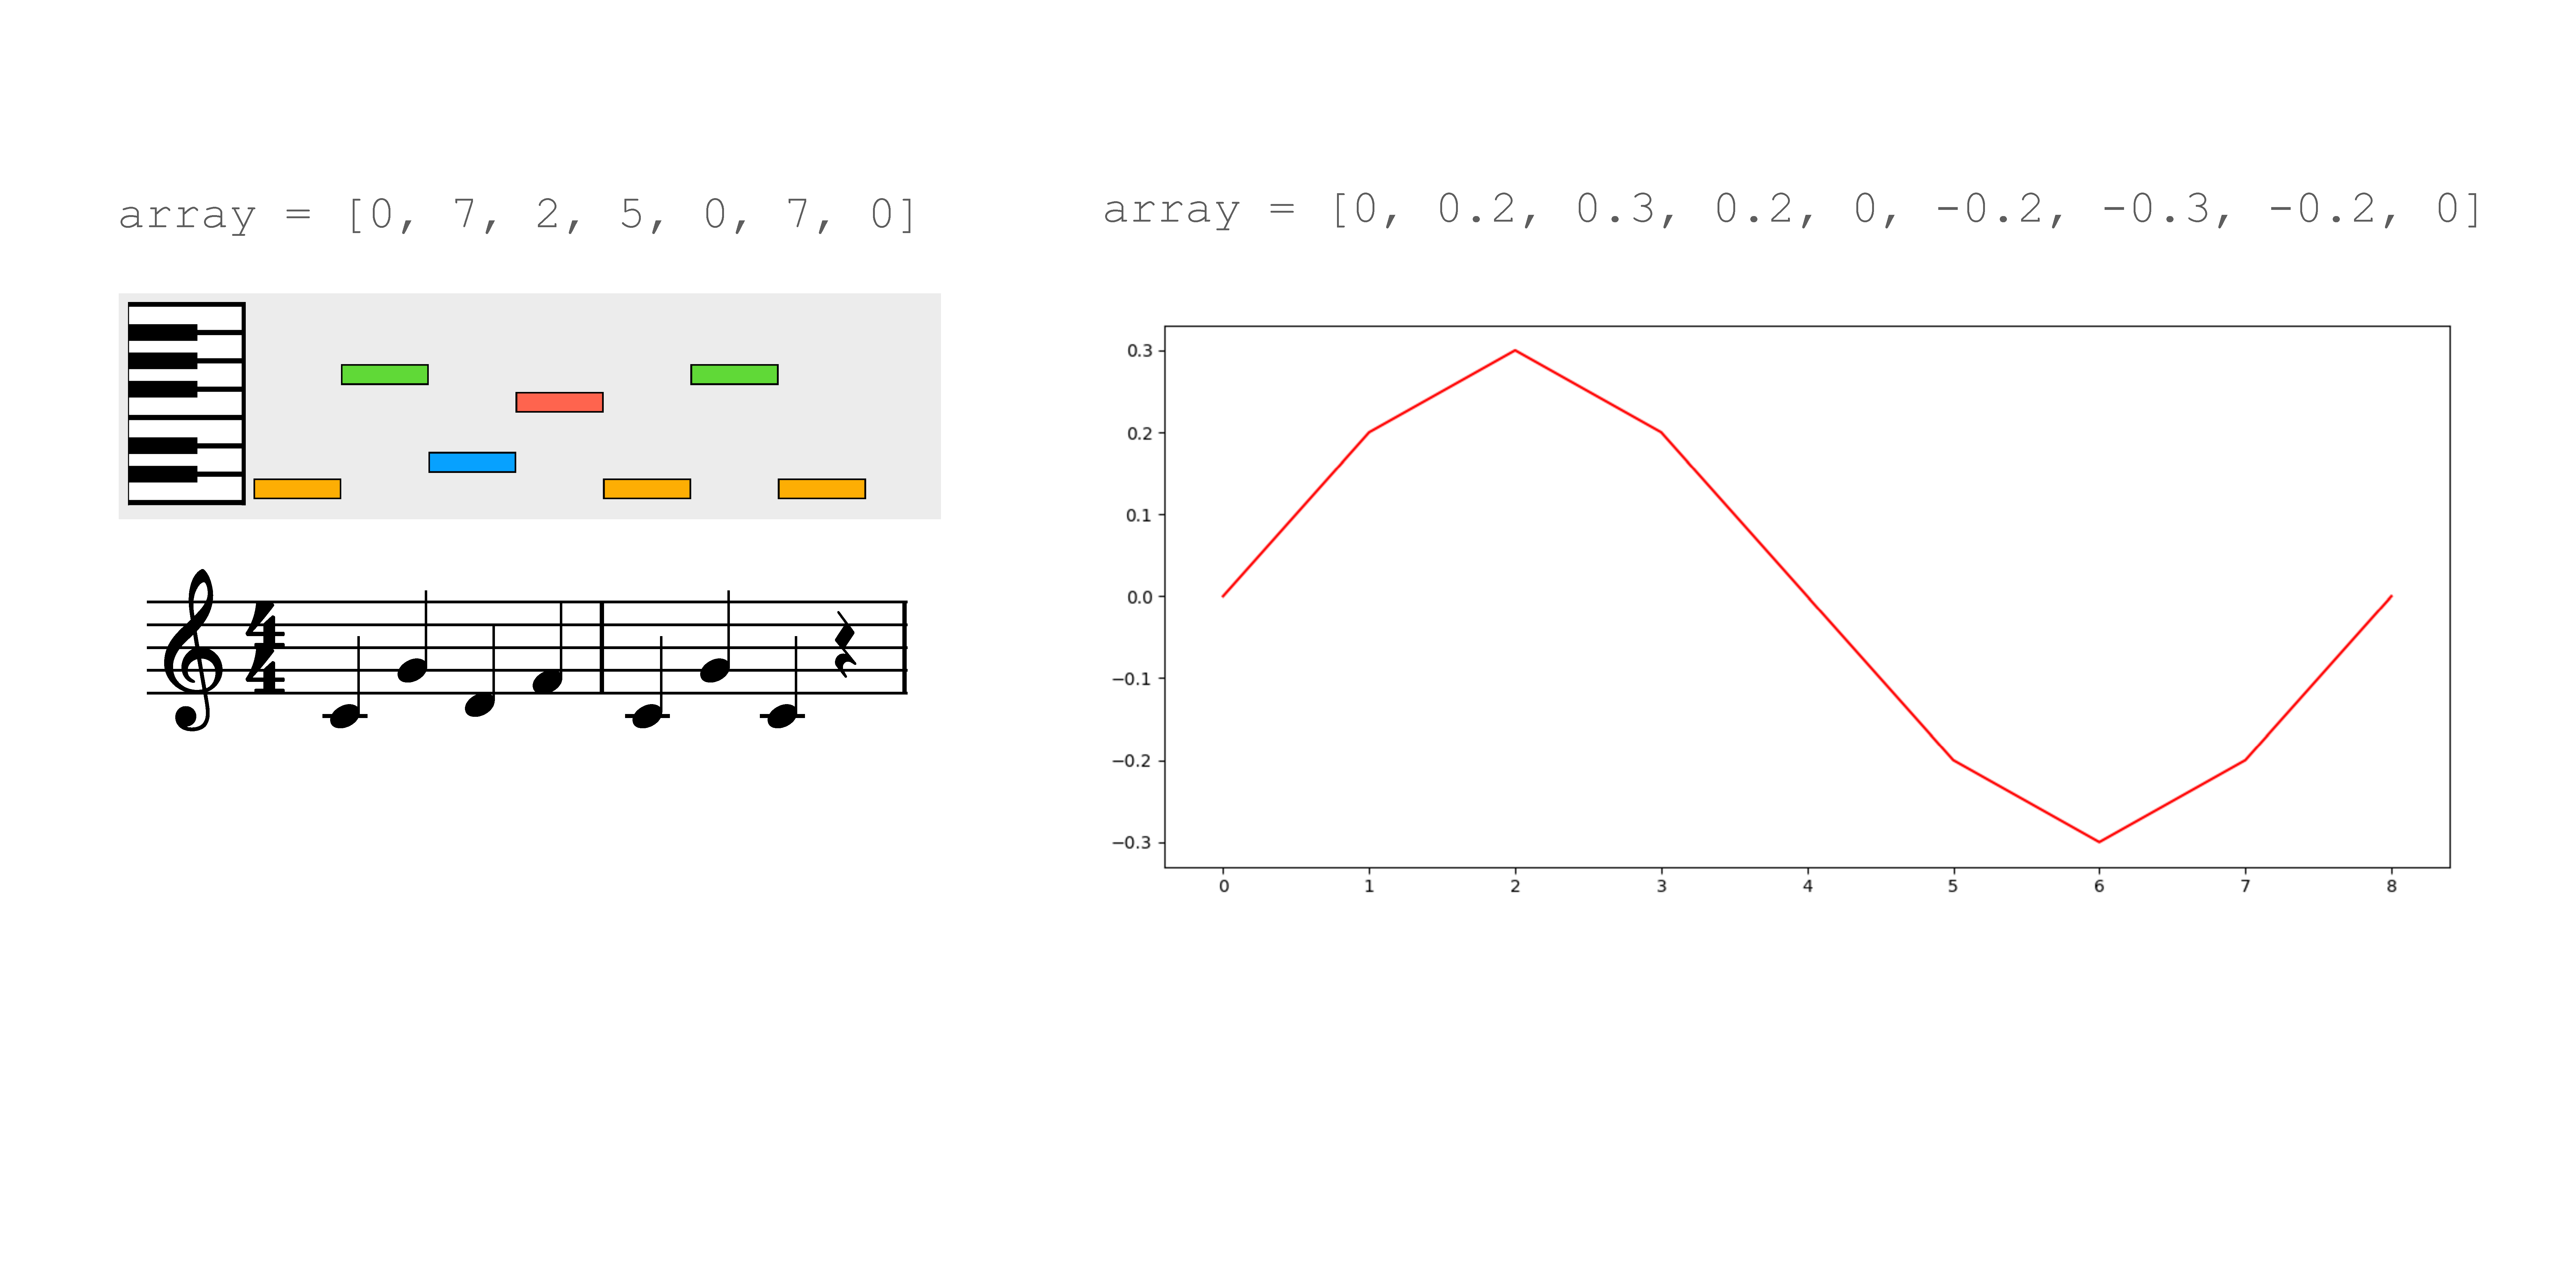
\includegraphics[width=1\linewidth]{images/fig1_arrays_as_sound_and_music.pdf}
    \caption{Two examples of arrays becoming sound and music. On the left, the array is translated into note values. On the right, the array is translated directly to an audio file.}
    \label{fig:arrays-as-music}
\end{figure}

interesting parallels with music and code anyway: scores are instructions too.

Rhythm and pitch - tailor made for iteration, conditionals, etc.

Music to teach/engage with simulation (Mike, Charlotte). Fourier transform as a nice transferable example...

Examples:
\begin{enumerate}
    \item Fourier transform
    \item Wave interference
    \item Resonance cavities $\leftrightarrow{}$ Guitars
    \item Oscillators, coupled oscillators (Idea of pendulums that make sound. Need to increase corresponding frequency to make it audible.)
\end{enumerate}


\section{Overview of what exists already} \label{sec:literature}
%Also quite brief, but pointing towards lots of existing work around
 %- introducing people to programming through music
% - introducing people to music through programming

Music and programming have been connected in a wide variety of ways, sometimes through the addition of libraries for integrating musical inputs and outputs with existing languages, and sometimes through the development of specifically designed languages or environments. As this is a very short chapter, it only scratches the surface of many of the interesting work done in this domain, with a particular emphasis on pedagogical elements.

Most mainstream programming languages are able to work with sound and music as outputs. This could be achieved by writing to a file, e.g. an audio file [NOD TO RESOURCES], a MIDI file (a common musical data format that can be used to synthesise sound). The program could also transmit real-time messages to an audio engine that runs separately, e.g. a standalone synthesiser or sampler \footnote{Lots of open source synthesisers are available such as \href{https://surge-synthesizer.github.io/}{Surge XT} or \href{https://asb2m10.github.io/dexed/}{Dexed}}, a digital audio workstation, or frameworks such as SuperDirt. In many cases there are existing libraries to achieve this. This makes it relatively easy to adapt any simple programming exercise to a sonic/musical exercise, e.g. adding an element to array could be adding a note to a melody or conditional statements might be musical decisions.

TOM QUESTION: COULD WE COMPILE A HANDY LIST OF EXAMPLE LIBRARIES FOR DIFFERENT LANGUAGES? I'M THINKING OF THINGS LIKE THIS IN PARTICULAR, WHERE IT MAY NOT BE OBVIOUS THAT THERE IS A WAY TO DO MUSICAL THINGS IN A GIVEN CONTEXT:
\href{https://flujoo.github.io/gm/articles/gm.html}{https://flujoo.github.io/gm/articles/gm.html}


Sonic Pi\footnote{\url{https://sonic-pi.net}} is a popular example of a specifically designed language: a simple but flexible environment that aims to support school-age students to learn to code by making music \cite{aaron_sonic_2016}. The focus on play and having fun with Sonic Pi can foster a more positive attitude towards programming \cite{petri_sonicpi_2022}, and can provide a starting point for moving from simple programming concepts to more involved topics such as concurrency \cite{traversaro_hearplay_2024}. Sound making programs can start off very simple with basic commands such as "play 60", but can be built into entire pieces or performances \cite{}. 

Sonic Pi is rooted in practices of live coding for music, a substantial community that serves as an access point to programming for many musicians, as well as an access point for music for some programmers. There  movement that has engaged closely with programming pedagogy from different perspectives. Blackwell et al \cite{blackwell_livecoding_2022} provide a useful overview of the field. The proceedings of the International Conference on Live Coding\footnote{\url{https://iclc.toplap.org/}} provide a more broader repository of topics, many of which cover music in programming education. Live musical coding is also notable as a community that has attempted to push back against coding as a male dominated space \cite{blackwell_livecoding_2022}, with all-women and non-binary workshops being a regular occurrence. Armitage \cite{armitage_spaces_2018} points to the domain as being a ``a space in which to fail constructively''.

The EarSketch\footnote{\url{https://earsketch.gatech.edu/}} \cite{engelman_earsketch_2017} and TunePad\footnote{\url{https://tunepad.com/}} projects are similar to Sonic Pi in their pedagogical aims, in that they seek to broaden participation in computing by demystifying coding and relating it to a domain of interest to students. The projects integrate coding into a digital audio workstation (DAW) framework that runs in a web browser, providing familiar workspaces for those with musical backgrounds. Both projects use Python (although EarSketch has a JavaScript option). They are designed specifically with sharing in mind: both code sharing and collaborative editing, further motivating students to engage with the coding \cite{freeman_earsketch_2019}. Petrie \cite{petrie_ct_2024} studied the potential for both projects to support computational thinking in 11-12 year old students who had no prior school experience of either programming or music making. Petrie notes how the kinds of musical tasks supported by these kinds of projects are naturally incremental and iterative, and that students benefit from that aspect.

STRUDEL / TIDALCYCLES


A key concern across all the above projects is that there should be room for musical variety and expression; although they may present simple entry points to engaging with programming, it is possible to create rich and interesting creative work that students will be proud of.

% NOTE: zoom out, make this broader, point to any other key literature areas

Some relevant references:
\begin{enumerate}
\item Creativity in CS1: A Literature Review \cite{Sharmin2021}
\item Sonic Pi – performance in education, technology and art \cite{Aaron2016}
\item \href{https://www.raspberrypi.org/app/uploads/2021/11/Teaching-programming-in-schools-pedagogy-review-Raspberry-Pi-Foundation.pdf}{Waite, Jane, and Sue Sentance. "Teaching programming in schools: A review of approaches and strategies." Raspberry Pi Foundation (2021).}
\item Live Coding book - Blackwell et al 2022
\item Earsketch, e.g. Freeman et al 2019
\item Computational thinking with EarSketch and TunePad: \url{https://www.tandfonline.com/doi/full/10.1080/08993408.2023.2240657#d1e252}
\item Music in R: \href{https://flujoo.github.io/gm/articles/gm.html}{https://flujoo.github.io/gm/articles/gm.html}
\item Benefits of integrating arts into STEM (STEAM): \href{https://doi.org/10.1016/j.procs.2013.09.317}{https://doi.org/10.1016/j.procs.2013.09.317}
\end{enumerate}

More projects specifically in the music/coding/pedagogy mould:
 - JythonMusic \url{https://intellectdiscover.com/content/journals/10.1386/jmte.9.1.33_1}

 This section is primarily about where education, music and programming come together.


 There is a substantial musical live coding community that serves as an access point to programming for many, as well as an access point for music for some programmers.


% REDUNDANT - recycle/remove
A wide variety of bespoke languages and tools have sprung up in relation to this, often building on top of the SuperCollider environment (CITE). Sonic Pi is particularly notable for being explicitly designed to support the teaching of programming \textbackslash{}cite\{Aaron16\}, particularly in schools for younger students. Live coding for music is often taught in a short workshop context \textbackslash{}cite\{Blackwell2022\}).



\section{Overview of our online resources [rename this]} \label{sec:resources}
%What are they, who are they for, what kinds of programming concepts do they relate to?

% Our working list of projects is here:
% https://docs.google.com/document/d/1FsmVMrJlf2lRL4Jb25oat9y6M3Uvrkz7JEuytC6oyb8/edit?usp=sharing

Include a list of resources for how you might adapt some of these examples to other libraries:
E.g. midi library things, audio read/write libraries, etc.
Other guides to setting up where these exist already.

Perhaps a quick note towards the many many things that are important, but perhaps out of scope here.

Each example resource comes with a readme that gives a sense of how the resource might be used, who might find it valuable, what prior knowledge the students may need, and what technologies will be needed.

\subsection{Python piano piece}
This resource is aimed at students who have started on Python quite recently. Students are shown how to generate piano pieces as MIDI data which can be played back directly within a Python notebook. Students can develop their understanding of fundamental concepts programming concepts such as lists, loops and conditionals. The ability to directly hear the results is intended to motivate students to think about how they can develop the code by themselves to try to explore how they can start to tailor the musical output towards something they find sonically interesting or satisfying.

\subsection{Strudel drum patterns}
This resource is both similar and different to the piano example. Students engage with \emph{Strudel}\footnote{\url{https://strudel.cc/workshop/getting-started/\#what-is-strudel}}, a browser-based JavaScript port of the popular \emph{TidalCycles}\footnote{https://tidalcycles.org/} live coding language. The language has been particularly popular for exploring algorithmic approaches to beat making\footnote{see the international Algorave movement for example: \url{https://algorave.com/}}. The editor provides useful visual feedback to show how the code relates to the unfolding beats. It has been a popular way to engage with code for the first time for many \ref{CITATION}, as well as being an useful introduction to Haskell and functional programming for others \cite{CITATION}. Unlike the Python example above, it may not be so straightforward to map programming insights directly to other domains such as data science or INSERT ANOTHER DOMAIN HERE.

\subsection{[Charlotte]}
% Short overview goes here
% 

\subsection{[Matthew]}
This section focusses on educators directly and the ground work needed to make the most portable and technologically accessible lessons. No prior knowledge is assumed and as the resource is intended to guide the reader through the process of WAVE file creation. The ultimate goal being a simple library ripe for customisation and intimately understood for easy dissemination to students.

All data can be a sound and the WAVE file is the simplest means of data sonification and music creation. Most modern operating systems (and many older ones) will support WAVE file playback through a media player, browser or command line tool. The resource emphasises the use of standard libraries to improve portability and providing a means of quickly beginning music-based programming lessons without burdening students with language-specific ancillary concepts that can potentially be a demotivating obstacle to new programmers.

The intention is not to be prescriptive, but rather show how malleable the WAVE format can be for teaching music and programming.

% want to talk about twos compliment? great, talk about signed integers and bit-depth. Want to talk about additivie synthesis? lovley, stack sine waves and put them in a .wav. Want to talk about Redbook audio, CD formats and PCM?  I wanetd emphasise here just how customusable such a simple basic concept (in computer science terms) and is stil very relevant. Basically almost like the WAVE file isn't the important bit, but the philosophy behind the decisions for teaching it.

The central lesson is explained in an IPython (Jupyter) notebook, but there is also companion code in C, C++, Java and Rust to reinforce the basic elements need to solve the problem.

% list of places to go, adding functionality to the library or expanding on the base WAVE format to include other chunks such as cue and playlist chunks which could be used in conjunction with reaper https://www.mmsp.ece.mcgill.ca/Documents/AudioFormats/WAVE/Docs/riffmci.pdf

\subsection{[Mike]}
% Short overview goes here

\subsection{[Yash]}
% Short overview goes here


\section{Mini summary}
Close it with a quick summary

Test writing permissions
